\documentclass{article}

% NeurIPS 2023 style (course template). neurips_2023.sty must be in the same folder.
% [preprint] shows author names (no anonymization, no line numbers).
% \usepackage[preprint]{neurips_2023}
\usepackage[utf8]{inputenc}
\usepackage[T1]{fontenc}
\usepackage{lmodern}
\providecommand{\And}{\and}
\renewcommand{\And}{\and}
\usepackage{hyperref}
\usepackage{url}
\usepackage{booktabs}
\usepackage{amsfonts,amsmath}
\usepackage{nicefrac}

\usepackage{xcolor}
\usepackage{graphicx}
\usepackage{multirow}

\renewcommand{\And}{\and}
\title{Does Salary Disclosure Have a Different Association with Job-Posting Engagement Across Career Levels?\\[4pt]
\large DS502/MA543 Final Project --- Group 4 --- Progress Report}

\author{%
  Aditya Jambhale 
  \And
  Vansh Patel 
  \And
  Syeda Tamzida Akter \\ Worcester Polytechnic Institute
}

\begin{document}
\maketitle

\begin{abstract}
We study whether LinkedIn job postings that disclose salary receive more engagement (views and applications) than postings that do not, and whether that association differs by career level. Using 123,849 postings from the LinkedIn Job Postings (2023--2024) dataset, we built a salary-disclosure indicator, log-transformed the heavily skewed engagement outcomes, and fit multiple linear regression with a disclosure~$\times$~career-level interaction, alongside Ridge and Lasso. After controlling for work type, remote status, application type, posting age, description length, region, and industry, disclosing postings receive about 10\% more views and 8\% more applications. For views, the association grows with seniority, from $+6\%$ at entry level to $+36\%$ at executive level (joint test of interactions $p=0.005$); for applications the same pattern appears but is not statistically significant ($p=0.19$). Regularization does not improve out-of-sample error (CV $R^2\approx0.15$--$0.17$ for all full models). We describe the main obstacles, which are non-random missingness in applications, unequal exposure time, and confounding by pay-transparency laws, and our plan to address them.
\end{abstract}

%=====================================================================
\section{Dataset and preprocessing}
\label{sec:data}

\paragraph{Source.} We use the Kaggle \emph{LinkedIn Job Postings (2023--2024)} dataset (\texttt{postings.csv}, 123,849 rows, 31 columns), joined with the auxiliary \texttt{job\_industries.csv} and \texttt{industries.csv} mapping tables. Postings were scraped over a short window in April 2024, so each row is a snapshot of cumulative engagement at scrape time.

\paragraph{Outcome variables.} \textbf{Views} are recorded for 98.6\% of postings. \textbf{Applications} (\texttt{applies}) are recorded for only 18.8\%. Both are extremely right-skewed: views have median 4, 99th percentile 177 and maximum 9,975 (skewness 53.7), and applications have median 3 and 99th percentile 134 (skewness 9.4). Neither outcome contains zeros. We model $\log(1+y)$, which reduces skewness to 1.87 (views) and 1.25 (applications) (Figure~\ref{fig:dist}). Coefficients on the log scale are reported as percentage differences, $100(e^{\beta}-1)$.

\begin{figure}[h]
  \centering
  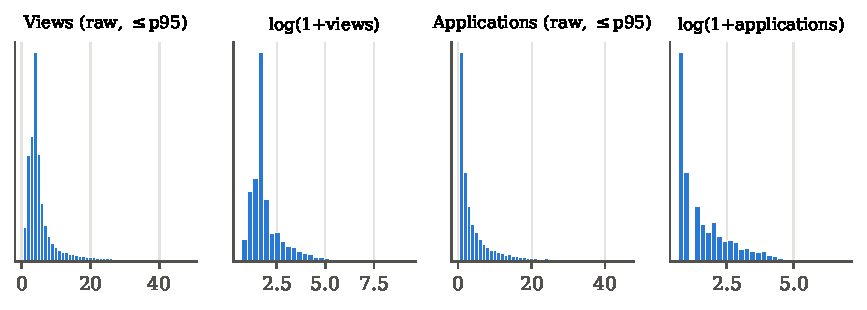
\includegraphics[width=\linewidth]{figures/fig1_distributions.pdf}
  \caption{Raw engagement (truncated at the 95th percentile for display) is extremely right-skewed; $\log(1+y)$ is much closer to symmetric.}
  \label{fig:dist}
\end{figure}

\paragraph{Main predictor.} \texttt{disclosed}~$=1$ if the posting has a non-missing normalized (annualized) salary. Of all postings, 29.1\% (36,073) disclose. Disclosures are annual (20,628), hourly (14,741) or other periods (704), and are almost entirely in USD.

\paragraph{Career level.} \texttt{formatted\_experience\_level} has six categories (Internship, Entry, Associate, Mid-Senior, Director, Executive) and is missing for 23.7\% of postings. The main analysis keeps the 94,440 postings with a known level and uses Entry as the reference category. Postings with an unspecified level are kept as their own category in a sensitivity check (§\ref{sec:results}).

\paragraph{Engineered controls.}
\begin{itemize}
  \item \textbf{Posting age} (exposure): days between \texttt{original\_listed\_time} and the latest listing timestamp in the data (the scrape snapshot), entered as $\log(1+\text{days})$ (median 2.1 days).
  \item \textbf{Work type}: Full-time, Part-time, Contract, Internship and Other (Temporary, Volunteer and Other merged).
  \item \textbf{Remote}: missing values set to 0, because the column only flags remote postings.
  \item \textbf{Application type}: Complex onsite, Simple onsite and Offsite.
  \item \textbf{Region}: US Census region parsed from the two-letter state in \texttt{location}, with an Unknown/National category for postings listed only as ``United States'' or a metro area.
  \item \textbf{Industry}: first listed industry, top 12 categories plus Other.
  \item \textbf{Description length}: $\log(1+\text{characters})$.
\end{itemize}
The \texttt{sponsored} flag is constant (all 0), so we dropped it.

\paragraph{Analysis samples.} Views: $n=93{,}227$; applications: $n=16{,}637$ (complete cases with known level).

%=====================================================================
\section{Methods implemented}
\label{sec:methods}

\paragraph{Inferential models (OLS).} For $y\in\{\log(1+\text{views}),\log(1+\text{applies})\}$ we fit three nested models:
\begin{align*}
\text{M0:}\quad & y = \beta_0 + \beta_1\,\text{disclosed} + \varepsilon\\
\text{M1:}\quad & y = \beta_0 + \beta_1\,\text{disclosed} + \textstyle\sum_\ell \gamma_\ell\,\text{level}_\ell + \mathbf{x}^\top\boldsymbol\delta + \varepsilon\\
\text{M2:}\quad & \text{M1} + \textstyle\sum_{\ell\neq\text{Entry}} \theta_\ell\,(\text{disclosed}\times\text{level}_\ell)
\end{align*}
where $\mathbf{x}$ contains the controls above (31 and 36 model degrees of freedom for M1 and M2). The disclosure association at level $\ell$ is $\beta_1+\theta_\ell$. Large employers post many similar ads, so standard errors are \textbf{clustered by company}. We test effect heterogeneity with a joint Wald test of $H_0:\theta_\ell=0\ \forall\ell$.

\paragraph{Predictive comparison.} We compare a mean-only baseline, OLS M0/M1/M2, \textbf{Ridge} and \textbf{Lasso} (on the M2 design, standardized features) using 5-fold cross-validation (seed 502), reporting RMSE, MAE and $R^2$ on the log scale. The Ridge penalty is chosen from 30 values in $[10^{-3},10^4]$ by efficient leave-one-out CV inside each training fold. The Lasso penalty is chosen by an inner 5-fold CV over 40 values. Regularized models are mainly used to test whether the interaction terms carry predictive signal, i.e., whether Lasso keeps them.

Implementation: Python (\texttt{pandas}, \texttt{statsmodels}, \texttt{scikit-learn}, \texttt{matplotlib}).

%=====================================================================
\section{Preliminary results}
\label{sec:results}

\paragraph{Who discloses?} Disclosure rates vary by level (Figure~\ref{fig:levels}a): lowest for Entry (24.9\%) and Internship (26.1\%), highest for Associate (39.6\%). Unadjusted, disclosing postings have higher mean $\log(1+\text{views})$ at every level, and the gap is visibly wider for Director and Executive roles (Figure~\ref{fig:levels}b). Raw medians differ by at most one view, so the differences come from the upper part of the distribution.

\begin{figure}[h]
  \centering
  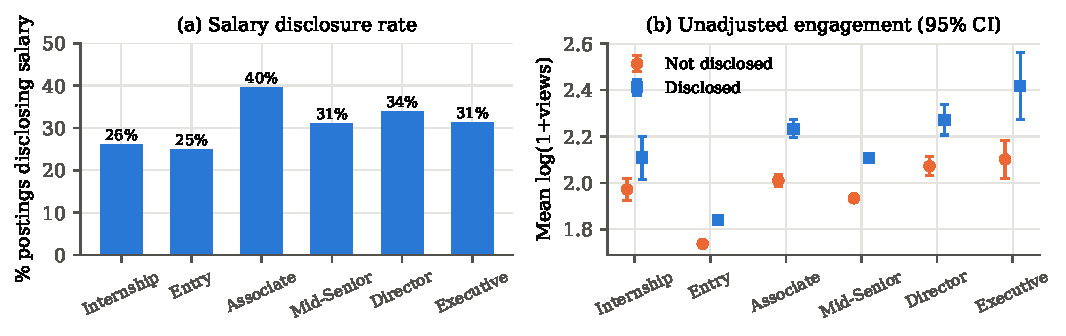
\includegraphics[width=\linewidth]{figures/fig2_levels.pdf}
  \caption{(a) Share of postings disclosing salary by career level. (b) Unadjusted mean $\log(1+\text{views})$ by disclosure status, with 95\% CIs.}
  \label{fig:levels}
\end{figure}

\paragraph{Overall association.} Table~\ref{tab:ols} summarizes the disclosure coefficient. Adding controls roughly halves the raw gap, which shows that disclosure is strongly confounded with posting characteristics. A clear association remains: about $+10\%$ views and $+8\%$ applications. Among the controls (M1), remote postings receive 46\% more views and 76\% more applications, offsite-apply postings receive 21\% fewer views and 31\% fewer recorded applications than complex onsite postings, and engagement rises with posting age as expected.

\begin{table}[h]
  \centering
  \caption{Disclosure coefficient on the log scale (company-clustered SE) and implied \% difference.}
  \label{tab:ols}
  \small
  \begin{tabular}{llcccc}
    \toprule
    Outcome & Model & $\hat\beta_{\text{disclosed}}$ (SE) & \% diff. & $R^2$ & $n$ \\
    \midrule
    \multirow{3}{*}{Views}
      & M0: disclosure only           & 0.182 (0.014) & $+20.0$ & 0.009 & \multirow{3}{*}{93,227} \\
      & M1: + level, controls         & 0.098 (0.016) & $+10.3$ & 0.151 & \\
      & M2: + interaction (Entry)     & 0.056 (0.014) & $+5.8$  & 0.152 & \\
    \midrule
    \multirow{3}{*}{Applications}
      & M0: disclosure only           & 0.148 (0.021) & $+16.0$ & 0.005 & \multirow{3}{*}{16,637} \\
      & M1: + level, controls         & 0.079 (0.018) & $+8.2$  & 0.170 & \\
      & M2: + interaction (Entry)     & 0.064 (0.033) & $+6.6$  & 0.171 & \\
    \bottomrule
  \end{tabular}
\end{table}

\paragraph{Heterogeneity across career levels.} Figure~\ref{fig:effects} shows the adjusted disclosure association at each level from M2. For \textbf{views} it rises steadily with seniority: Entry $+5.8\%$ [3.0, 8.7], Associate $+13.2\%$, Mid-Senior $+12.1\%$, Director $+16.5\%$, Executive $+35.7\%$ [12.6, 63.6]. The five interaction terms are jointly significant (Wald $\chi^2_5=16.9$, $p=0.005$). For \textbf{applications} the pattern is similar at the top (Director $+19.9\%$, Executive $+35.3\%$), but the intervals are wide and the joint test is not significant ($\chi^2_5=7.4$, $p=0.19$). This is consistent with the applications sample being about 5.6$\times$ smaller. The Internship estimate is imprecise for both outcomes.

\begin{figure}[h]
  \centering
  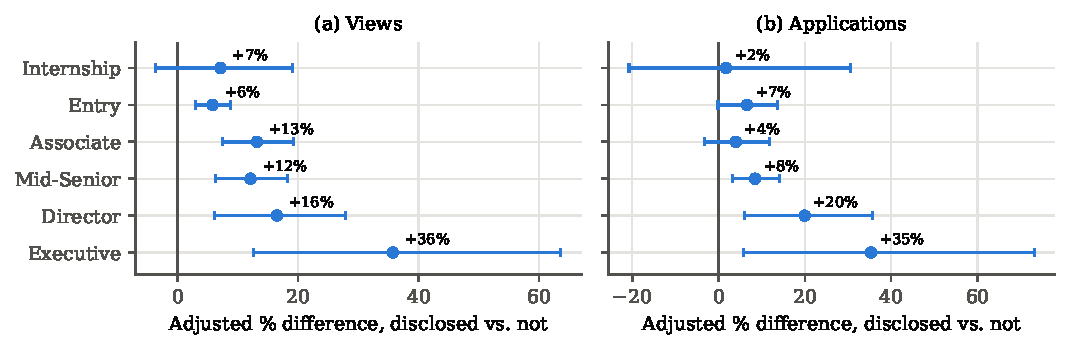
\includegraphics[width=\linewidth]{figures/fig3_level_effects.pdf}
  \caption{Adjusted \% difference in engagement for disclosing vs.\ non-disclosing postings at each career level (M2, $\beta_1+\theta_\ell$, 95\% company-clustered CIs).}
  \label{fig:effects}
\end{figure}

\paragraph{Predictive performance and regularization.} Table~\ref{tab:cv} and Figure~\ref{fig:cv} report the 5-fold CV results. Disclosure alone explains under 1\% of variance. The controls lift CV $R^2$ to about 0.15 (views) and 0.17 (applications). The interaction adds essentially nothing to prediction ($\Delta R^2 \le 0.0003$), even though it is statistically detectable for views. The effect is real but small relative to the noise in individual engagement. Ridge matches OLS, because with $n\gg p$ (36 features) there is little variance to reduce. For views, Lasso selects a tiny penalty ($\alpha=4\times10^{-4}$) and keeps all 36 features, including every interaction (shrunk). For applications, Lasso ($\alpha=0.018$) zeroes 19 of 36 features, dropping all interactions except Executive while keeping the main disclosure term, which matches the inferential result above.

\begin{table}[h]
  \centering
  \caption{5-fold cross-validated performance on the log scale (mean over folds; SD of $R^2$ in parentheses).}
  \label{tab:cv}
  \small
  \begin{tabular}{lccc@{\hspace{14pt}}ccc}
    \toprule
    & \multicolumn{3}{c}{$\log(1+\text{views})$} & \multicolumn{3}{c}{$\log(1+\text{applications})$} \\
    \cmidrule(lr){2-4}\cmidrule(lr){5-7}
    Model & RMSE & MAE & $R^2$ & RMSE & MAE & $R^2$ \\
    \midrule
    Mean baseline          & 0.870 & 0.599 & 0.000 (0.000) & 1.053 & 0.836 & $-0.001$ (0.001) \\
    OLS M0                 & 0.866 & 0.597 & 0.009 (0.001) & 1.050 & 0.835 & 0.003 (0.003) \\
    OLS M1                 & 0.802 & 0.551 & 0.151 (0.002) & \textbf{0.961} & \textbf{0.747} & \textbf{0.165} (0.009) \\
    OLS M2                 & \textbf{0.801} & 0.551 & \textbf{0.151} (0.002) & 0.962 & 0.747 & 0.165 (0.009) \\
    Ridge (M2 design)      & \textbf{0.801} & 0.551 & \textbf{0.151} (0.002) & 0.962 & 0.747 & 0.165 (0.009) \\
    Lasso (M2 design)      & \textbf{0.801} & \textbf{0.551} & \textbf{0.151} (0.002) & 0.965 & 0.754 & 0.158 (0.007) \\
    \bottomrule
  \end{tabular}
\end{table}

\begin{figure}[h]
  \centering
  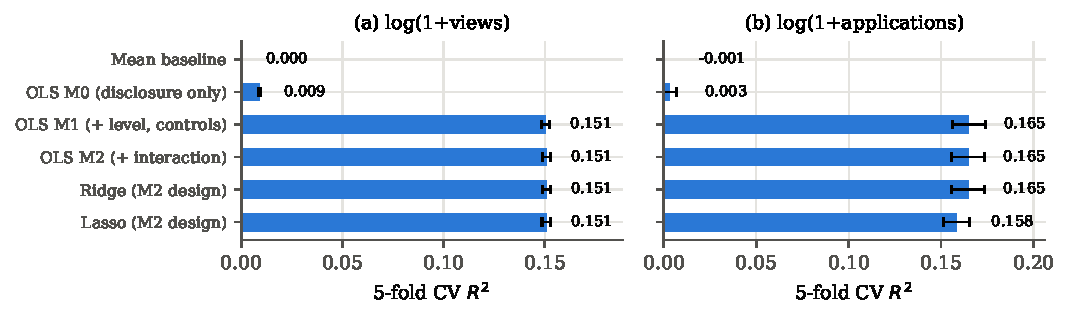
\includegraphics[width=\linewidth]{figures/fig4_cv.pdf}
  \caption{5-fold CV $R^2$ (error bars: SD across folds). Controls carry the predictive signal; regularization and the interaction do not change accuracy.}
  \label{fig:cv}
\end{figure}

\paragraph{Sensitivity checks (views, M1).} (i) Keeping postings with an unspecified level as their own category ($n=122{,}160$) gives $\hat\beta=0.104$ (SE 0.014), i.e., $+11.0\%$, essentially unchanged. (ii) Comparing only annual-salary disclosures against non-disclosing postings ($n=80{,}961$) gives a larger association, $\hat\beta=0.155$ (SE 0.022), i.e., $+16.8\%$. This suggests that \emph{how} pay is disclosed (annual vs.\ hourly) matters and needs a closer look.

%=====================================================================
\section{Challenges and plan to address them}
\label{sec:challenges}

\begin{enumerate}
  \item \textbf{Applications are missing not at random.} \texttt{applies} is recorded for 37.5\% of complex-onsite, 23.8\% of simple-onsite and only 11.5\% of offsite-apply postings. Offsite applications happen on employer sites and are mostly untracked. The applications model therefore describes a selected subsample. \emph{Plan:} report applications results separately by application type, fit a missingness model (logistic regression for ``applies observed'') to check whether disclosure itself predicts observation, and state the restricted scope clearly in the final report.
  \item \textbf{Unequal exposure.} Engagement is cumulative and most postings are only a few days old at the snapshot, so older postings mechanically have more views. \emph{Plan:} beyond the $\log(\text{age})$ control, model engagement \emph{rates} (views per day) and fit a Poisson / negative-binomial GLM with a $\log(\text{age})$ offset as a robustness check on the log-OLS results.
  \item \textbf{Confounding by pay-transparency laws.} Several states (e.g., CA, CO, NY, WA) require pay ranges in postings, so disclosure is partly determined by location, which may also affect engagement. Our current region control is coarse. \emph{Plan:} replace Census region with state fixed effects plus a pay-transparency-law indicator, and re-estimate within law states only, where disclosure is closer to mandatory.
  \item \textbf{Low explained variance.} CV $R^2\approx0.15$ shows that most engagement variation is idiosyncratic (job title, employer brand, timing). Since our goal is inference about an association, this is acceptable, but it limits predictive claims. \emph{Plan:} add title-based features (e.g., seniority keywords, TF-IDF top terms) and a nonlinear benchmark (random forest or gradient boosting) to check whether the linear specification misses structure.
  \item \textbf{Small senior-level cells.} Executive (1,222) and Internship (1,449) postings give wide intervals, especially for applications. \emph{Plan:} report these with appropriate caution and consider pooling Director and Executive as ``Senior leadership'' as a robustness check.
\end{enumerate}

%=====================================================================
\section{Updates to the original project plan}
\label{sec:updates}

Compared with our Phase~2 abstract:
\begin{itemize}
  \item \textbf{Additional controls.} We added posting age (exposure), description length, Census region and industry, because the raw disclosure gap halves once posting characteristics are controlled for.
  \item \textbf{Clustered inference.} Standard errors are clustered by company, because many companies post multiple similar jobs.
  \item \textbf{Defined scope for career level.} The main analysis uses the six known levels. Unspecified-level postings (23.7\%) enter only as a sensitivity check.
  \item \textbf{Role of Ridge/Lasso clarified.} With 36 features and tens of thousands of observations, regularization does not improve prediction. We now use Lasso primarily as a variable-selection check on the interaction terms, and plan to add a count-data GLM and a tree-based benchmark (§\ref{sec:challenges}).
  \item \textbf{New sub-question.} The annual-vs.-hourly sensitivity result suggests examining disclosure \emph{format}, and, among disclosers, the salary level itself.
\end{itemize}

\paragraph{Remaining timeline.} (1) Robustness: count GLM with offset, state and pay-transparency controls, missingness model. (2) Title features and nonlinear benchmark. (3) Final report and presentation.

%=====================================================================
\section*{Team contributions}
% TODO (team): replace with who did what.


\end{document}
